% Options for packages loaded elsewhere
\PassOptionsToPackage{unicode}{hyperref}
\PassOptionsToPackage{hyphens}{url}
\PassOptionsToPackage{dvipsnames,svgnames,x11names}{xcolor}
%
\documentclass[
  letterpaper,
  DIV=11,
  numbers=noendperiod,
  oneside]{scrartcl}

\usepackage{amsmath,amssymb}
\usepackage{lmodern}
\usepackage{iftex}
\ifPDFTeX
  \usepackage[T1]{fontenc}
  \usepackage[utf8]{inputenc}
  \usepackage{textcomp} % provide euro and other symbols
\else % if luatex or xetex
  \usepackage{unicode-math}
  \defaultfontfeatures{Scale=MatchLowercase}
  \defaultfontfeatures[\rmfamily]{Ligatures=TeX,Scale=1}
\fi
% Use upquote if available, for straight quotes in verbatim environments
\IfFileExists{upquote.sty}{\usepackage{upquote}}{}
\IfFileExists{microtype.sty}{% use microtype if available
  \usepackage[]{microtype}
  \UseMicrotypeSet[protrusion]{basicmath} % disable protrusion for tt fonts
}{}
\makeatletter
\@ifundefined{KOMAClassName}{% if non-KOMA class
  \IfFileExists{parskip.sty}{%
    \usepackage{parskip}
  }{% else
    \setlength{\parindent}{0pt}
    \setlength{\parskip}{6pt plus 2pt minus 1pt}}
}{% if KOMA class
  \KOMAoptions{parskip=half}}
\makeatother
\usepackage{xcolor}
\usepackage[left=1in,marginparwidth=2.0666666666667in,textwidth=4.1333333333333in,marginparsep=0.3in]{geometry}
\setlength{\emergencystretch}{3em} % prevent overfull lines
\setcounter{secnumdepth}{-\maxdimen} % remove section numbering
% Make \paragraph and \subparagraph free-standing
\ifx\paragraph\undefined\else
  \let\oldparagraph\paragraph
  \renewcommand{\paragraph}[1]{\oldparagraph{#1}\mbox{}}
\fi
\ifx\subparagraph\undefined\else
  \let\oldsubparagraph\subparagraph
  \renewcommand{\subparagraph}[1]{\oldsubparagraph{#1}\mbox{}}
\fi


\providecommand{\tightlist}{%
  \setlength{\itemsep}{0pt}\setlength{\parskip}{0pt}}\usepackage{longtable,booktabs,array}
\usepackage{calc} % for calculating minipage widths
% Correct order of tables after \paragraph or \subparagraph
\usepackage{etoolbox}
\makeatletter
\patchcmd\longtable{\par}{\if@noskipsec\mbox{}\fi\par}{}{}
\makeatother
% Allow footnotes in longtable head/foot
\IfFileExists{footnotehyper.sty}{\usepackage{footnotehyper}}{\usepackage{footnote}}
\makesavenoteenv{longtable}
\usepackage{graphicx}
\makeatletter
\def\maxwidth{\ifdim\Gin@nat@width>\linewidth\linewidth\else\Gin@nat@width\fi}
\def\maxheight{\ifdim\Gin@nat@height>\textheight\textheight\else\Gin@nat@height\fi}
\makeatother
% Scale images if necessary, so that they will not overflow the page
% margins by default, and it is still possible to overwrite the defaults
% using explicit options in \includegraphics[width, height, ...]{}
\setkeys{Gin}{width=\maxwidth,height=\maxheight,keepaspectratio}
% Set default figure placement to htbp
\makeatletter
\def\fps@figure{htbp}
\makeatother
\newlength{\cslhangindent}
\setlength{\cslhangindent}{1.5em}
\newlength{\csllabelwidth}
\setlength{\csllabelwidth}{3em}
\newlength{\cslentryspacingunit} % times entry-spacing
\setlength{\cslentryspacingunit}{\parskip}
\newenvironment{CSLReferences}[2] % #1 hanging-ident, #2 entry spacing
 {% don't indent paragraphs
  \setlength{\parindent}{0pt}
  % turn on hanging indent if param 1 is 1
  \ifodd #1
  \let\oldpar\par
  \def\par{\hangindent=\cslhangindent\oldpar}
  \fi
  % set entry spacing
  \setlength{\parskip}{#2\cslentryspacingunit}
 }%
 {}
\usepackage{calc}
\newcommand{\CSLBlock}[1]{#1\hfill\break}
\newcommand{\CSLLeftMargin}[1]{\parbox[t]{\csllabelwidth}{#1}}
\newcommand{\CSLRightInline}[1]{\parbox[t]{\linewidth - \csllabelwidth}{#1}\break}
\newcommand{\CSLIndent}[1]{\hspace{\cslhangindent}#1}

\KOMAoption{captions}{tableheading}
\makeatletter
\makeatother
\makeatletter
\makeatother
\makeatletter
\@ifpackageloaded{caption}{}{\usepackage{caption}}
\AtBeginDocument{%
\ifdefined\contentsname
  \renewcommand*\contentsname{Table of contents}
\else
  \newcommand\contentsname{Table of contents}
\fi
\ifdefined\listfigurename
  \renewcommand*\listfigurename{List of Figures}
\else
  \newcommand\listfigurename{List of Figures}
\fi
\ifdefined\listtablename
  \renewcommand*\listtablename{List of Tables}
\else
  \newcommand\listtablename{List of Tables}
\fi
\ifdefined\figurename
  \renewcommand*\figurename{Figure}
\else
  \newcommand\figurename{Figure}
\fi
\ifdefined\tablename
  \renewcommand*\tablename{Table}
\else
  \newcommand\tablename{Table}
\fi
}
\@ifpackageloaded{float}{}{\usepackage{float}}
\floatstyle{ruled}
\@ifundefined{c@chapter}{\newfloat{codelisting}{h}{lop}}{\newfloat{codelisting}{h}{lop}[chapter]}
\floatname{codelisting}{Listing}
\newcommand*\listoflistings{\listof{codelisting}{List of Listings}}
\makeatother
\makeatletter
\@ifpackageloaded{caption}{}{\usepackage{caption}}
\@ifpackageloaded{subcaption}{}{\usepackage{subcaption}}
\makeatother
\makeatletter
\@ifpackageloaded{tcolorbox}{}{\usepackage[many]{tcolorbox}}
\makeatother
\makeatletter
\@ifundefined{shadecolor}{\definecolor{shadecolor}{rgb}{.97, .97, .97}}
\makeatother
\makeatletter
\@ifpackageloaded{sidenotes}{}{\usepackage{sidenotes}}
\@ifpackageloaded{marginnote}{}{\usepackage{marginnote}}
\makeatother
\makeatletter
\makeatother
\ifLuaTeX
  \usepackage{selnolig}  % disable illegal ligatures
\fi
\IfFileExists{bookmark.sty}{\usepackage{bookmark}}{\usepackage{hyperref}}
\IfFileExists{xurl.sty}{\usepackage{xurl}}{} % add URL line breaks if available
\urlstyle{same} % disable monospaced font for URLs
\hypersetup{
  pdftitle={Nanoparticulate Drug Delivery Systems},
  pdfauthor={Rhys McAlister},
  colorlinks=true,
  linkcolor={blue},
  filecolor={Maroon},
  citecolor={Blue},
  urlcolor={Blue},
  pdfcreator={LaTeX via pandoc}}

\title{Nanoparticulate Drug Delivery Systems}
\usepackage{etoolbox}
\makeatletter
\providecommand{\subtitle}[1]{% add subtitle to \maketitle
  \apptocmd{\@title}{\par {\large #1 \par}}{}{}
}
\makeatother
\subtitle{A summary of a series of lectures on nanoparticulate drug
delivery systems for cancer therapy.}
\author{Rhys McAlister}
\date{2022/10/22}

\begin{document}
\maketitle
\ifdefined\Shaded\renewenvironment{Shaded}{\begin{tcolorbox}[interior hidden, borderline west={3pt}{0pt}{shadecolor}, sharp corners, enhanced, breakable, frame hidden, boxrule=0pt]}{\end{tcolorbox}}\fi

\renewcommand*\contentsname{Table of contents}
{
\hypersetup{linkcolor=}
\setcounter{tocdepth}{2}
\tableofcontents
}
Work in progress document.

\hypertarget{why-are-nanoparticles-used-in-medicine}{%
\section{Why are nanoparticles used in
medicine?}\label{why-are-nanoparticles-used-in-medicine}}

Nanoparticles used for medicinal purposes are referred to as
nanomedicines and these agents have multi-dimensional usage as
diagnostic tools or vehicles used for the targeted delivery of selected
therapeutic compounds(Sadeghi et al. 2020). Nanoparticles are defined as
being between 1-100 nanometres (nm) in diameter and these particles have
already been used in the delivery of drugs such as vaccines, nucleotides
and recombinant proteins(Sadeghi et al. 2020). These nanoparticle
dependent delivery strategies exhibit improvements in rate of
absorption, reduction in elimination kinetics and controlled
release(Sadeghi et al. 2020).

Traditional drug administration normally involves the oral and
intravenous delivery of drug molecules. These drug particles travel in
an unguided manner and this results in a systemic distribution
throughout the body(Lu et al. 2021). It is instead desirable to have the
drug molecules primarily be located at the desired site of action as
this systemic distribution results in low drug efficacy and enhances the
potential for off target effects(Lu et al. 2021).

An important consideration within pharmacological treatments is how to
best maintain the concentration of the drug at the site of action. The
optimal concentration range is termed as the therapeutic window and this
window is a range in which the effectiveness of the drug is maintained
without reaching toxic levels. The use of nanoparticle delivery systems
allows for the pharmacokinetics and biodistribution of a drug to be
dependent upon the characteristics of a given nanoparticle and not upon
the drug molecule.

Nanoparticles have been constructed from various materials and the four
major compositional categories are: organic, inorganic, carbon-based and
composite-based(Jeevanandam et al. 2018). The material choice in
addition to the size and shape of the nanoparticle are key in
determining its biological outcomes(Jeevanandam et al. 2018). Additional
considerations are the particles surface bioactivity and functionality.

\begin{marginfigure}

{\centering 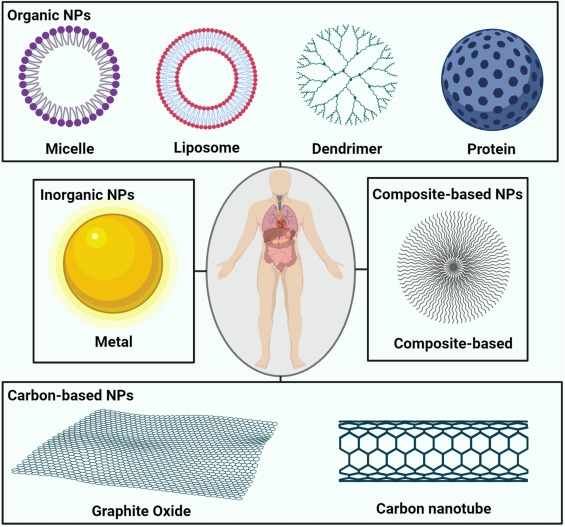
\includegraphics{cat-image.jpg}

}

\caption{Nanoparticle composition categories (Sadeghi et al. 2020)}

\end{marginfigure}

\hypertarget{biodistribution-of-nanoparticles}{%
\section{Biodistribution of
nanoparticles}\label{biodistribution-of-nanoparticles}}

Nanoparticles can be administered using various different routes (see
table 1), however the preeminent manner is intravenous administration
currently. The route of administration plays a large role in determining
the biodistribution of a nanoparticle and specific characteristics of
the particle can be tuned in order to have further control over the
specific site of deposition for a given particle. When nanoparticles are
inhaled, there is significant accumulation in the lung tissue, however
the diameter of the nanoparticle can critically determine the specific
site the particles will accumulate. Figure~\ref{fig-deposition}
demonstrates that particles (0.001-0.01 \(\mu\)m) can be seen to
accumulate significantly in the extra thoracic region whereas relatively
larger particles begin to accumulate more significantly in the
intrathoracic region(Geiser and Kreyling 2010).

\begin{figure}

{\centering \includegraphics{12989_2009_Article_100_Fig6_HTML.webp}

}

\caption{\label{fig-deposition}Particle deposition in the respiratory
tract.}

\end{figure}

\begin{longtable}[]{@{}
  >{\raggedright\arraybackslash}p{(\columnwidth - 4\tabcolsep) * \real{0.1157}}
  >{\raggedright\arraybackslash}p{(\columnwidth - 4\tabcolsep) * \real{0.4380}}
  >{\raggedright\arraybackslash}p{(\columnwidth - 4\tabcolsep) * \real{0.4463}}@{}}
\caption{Table 1. Comparison of routes of administration(Sadeghi et al.
2020)}\tabularnewline
\toprule()
\begin{minipage}[b]{\linewidth}\raggedright
Route
\end{minipage} & \begin{minipage}[b]{\linewidth}\raggedright
Advantages
\end{minipage} & \begin{minipage}[b]{\linewidth}\raggedright
Disadvantages/Challenges for nanoparticles
\end{minipage} \\
\midrule()
\endfirsthead
\toprule()
\begin{minipage}[b]{\linewidth}\raggedright
Route
\end{minipage} & \begin{minipage}[b]{\linewidth}\raggedright
Advantages
\end{minipage} & \begin{minipage}[b]{\linewidth}\raggedright
Disadvantages/Challenges for nanoparticles
\end{minipage} \\
\midrule()
\endhead
Oral & \begin{minipage}[t]{\linewidth}\raggedright
\begin{itemize}
\item
  Patient compliance
\item
  Fewer infections/contamination
\item
  Dosage flexibility
\item
  Extensive drug absorption area in the GI tract
\end{itemize}
\end{minipage} & \begin{minipage}[t]{\linewidth}\raggedright
\begin{itemize}
\item
  Acidic pH of the stomach
\item
  Presence of proteolytic enzymes in the GI tract
\item
  Low permeation across the intestinal epithelium
\end{itemize}
\end{minipage} \\
Nasal & \begin{minipage}[t]{\linewidth}\raggedright
\begin{itemize}
\item
  Large surface area particularly in the lungs
\item
  Highly vascularised mucosa
\item
  Porous endothelial membrane
\item
  Negligible enzymatic activity
\item
  Bypasses first-pass metabolism
\end{itemize}
\end{minipage} & \begin{minipage}[t]{\linewidth}\raggedright
\begin{itemize}
\item
  Size limited through the delivery device
\item
  Presence of nasal clearance
\item
  Proteolytic instability
\end{itemize}
\end{minipage} \\
Pulmonary & \begin{minipage}[t]{\linewidth}\raggedright
\begin{itemize}
\item
  Large absorption surface area
\item
  Significant vascularisation
\item
  Narrow alveolar epithelial membrane
\item
  Negligible enzymatic activity
\end{itemize}
\end{minipage} & \begin{minipage}[t]{\linewidth}\raggedright
\begin{itemize}
\item
  Can have an irritant effect on the airways
\item
  Protein and peptide degradation
\item
  Low retention of drug within the lungs
\end{itemize}
\end{minipage} \\
Intravenous & \begin{minipage}[t]{\linewidth}\raggedright
\begin{itemize}
\item
  Systemic delivery
\item
  Systemic action
\end{itemize}
\end{minipage} & \begin{minipage}[t]{\linewidth}\raggedright
\begin{itemize}
\item
  Invasive
\item
  Heptatotoxicity
\item
  Systemic toxicity
\end{itemize}
\end{minipage} \\
Ocular & \begin{minipage}[t]{\linewidth}\raggedright
\begin{itemize}
\item
  Ease of administration
\item
  Circumvents first-pass metabolism
\end{itemize}
\end{minipage} & \begin{minipage}[t]{\linewidth}\raggedright
\begin{itemize}
\item
  Poor permeability
\item
  Enzymatic degradation
\item
  Nasolacrimal drainage
\end{itemize}
\end{minipage} \\
\bottomrule()
\end{longtable}

\hypertarget{from-i.v-administration-to-the-cell}{%
\section*{From I.V administration to the
cell}\label{from-i.v-administration-to-the-cell}}
\addcontentsline{toc}{section}{From I.V administration to the cell}

\hypertarget{refs}{}
\begin{CSLReferences}{1}{0}
\leavevmode\vadjust pre{\hypertarget{ref-geiser2010}{}}%
Geiser, Marianne, and Wolfgang G Kreyling. 2010. {``Deposition and
Biokinetics of Inhaled Nanoparticles.''} \emph{Particle and Fibre
Toxicology} 7 (1): 2. \url{https://doi.org/10.1186/1743-8977-7-2}.

\leavevmode\vadjust pre{\hypertarget{ref-jeevanandam2018}{}}%
Jeevanandam, Jaison, Ahmed Barhoum, Yen S Chan, Alain Dufresne, and
Michael K Danquah. 2018. {``Review on Nanoparticles and Nanostructured
Materials: History, Sources, Toxicity and Regulations.''}
\emph{Beilstein Journal of Nanotechnology} 9 (April): 1050--74.
\url{https://doi.org/10.3762/bjnano.9.98}.

\leavevmode\vadjust pre{\hypertarget{ref-lu2021}{}}%
Lu, Weijia, Jing Yao, Xiao Zhu, and Yi Qi. 2021. {``Nanomedicines:
Redefining Traditional Medicine.''} \emph{Biomedicine \&
Pharmacotherapy} 134 (February): 111103.
\url{https://doi.org/10.1016/j.biopha.2020.111103}.

\leavevmode\vadjust pre{\hypertarget{ref-sadeghi2020}{}}%
Sadeghi, Samira, Wai Kit Lee, Shik Nie Kong, Annanya Shetty, and Chester
Lee Drum. 2020. {``Oral Administration of Protein Nanoparticles: An
Emerging Route to Disease Treatment.''} \emph{Pharmacological Research}
158 (August): 104685. \url{https://doi.org/10.1016/j.phrs.2020.104685}.

\end{CSLReferences}



\end{document}
